\documentclass{article}
\usepackage{tikz}
\usepackage[fleqn]{amsmath}
\usepackage{amsthm}
\usepackage{amssymb}

\title{Homework 8}
\author{John Carlyle}

\begin{document}
\maketitle

\begin{description}
  
\item[1.]\hfill \\
  \begin{description}
  \item[b.]
    \begin{align*}
      S \rightarrow&\: SS ~|~ bS ~|~ a\\
    \end{align*}
    $\{ x | ~x$ does not end in $b\}$
    
  \item[c.]
    \begin{align*}
      S \rightarrow&\: SaS ~|~ b\\
    \end{align*}
    $\{ x |~ x$ contains alternating $a$ and $b$ starting and ending with $b\}$
    
  \item[e.]
    \begin{align*}
      S \rightarrow& \: TT\\
      T \rightarrow& \: Ta ~|~ aT ~|~ b
    \end{align*}
    $\{x|~n_b(x) = 2\}$

  \item[f.]
    \begin{align*}
      S \rightarrow& \: aSa ~|~ bSb ~|~ aAb ~|~ bAa\\
      A \rightarrow& \: aAa ~|~ bAb ~|~ a ~|~ b ~|~ \lambda\\
    \end{align*}
    $\{ x | ~ x \ne aa, bb, \lambda \}$

  \item[g.]
    \begin{align*}
      S \rightarrow&~ aT ~|~ bT ~|~ \lambda\\
      T \rightarrow&~ aS ~|~ bS\\
    \end{align*}
    $\{x |~|x| = $ even $\}$

  \item[h.]
    \begin{align*}
      S \rightarrow&~ aT ~|~ bT\\
      T \rightarrow& \: aS ~|~ bS ~|~ \lambda\\
    \end{align*}
    $\{ x |~|x| = $ odd $ \} $

  \end{description}

\item[3.]\hfill \\
  \begin{description}
  \item[a.]
    The set of odd-length strings in $\{a,b\}^*$ with middle symbol $a$.
    \begin{align*}
      S \rightarrow&~ aSa ~|~ aSb ~|~ bSa ~|~ bSb ~|~ a\\
    \end{align*}

  \item[b.]
    The set of even-length strings in $\{a,b\}^*$ with two middle symbols equal.
    \begin{align*}
      S \rightarrow&~ aSa ~|~ aSb ~|~ bSa ~|~ bSb ~|~ aa ~|~ bb\\
    \end{align*}
    
  \item[c.]
    The set of odd-length strings in $\{a,b\}^*$ whose first, middle and last symbols are the same.
    \begin{align*}
      S \rightarrow&~ aAaAa ~|~ bAbAb ~|~ a ~|~ b\\
      A \rightarrow&~ aA ~|~ bA ~|~ \lambda\\
    \end{align*}
  \end{description}

\item[4.]\hfill \\
  \begin{description}
  \item[a.]\hfill \\
    Let $G$ be the grammar defined by $S \rightarrow SabS ~|~ SbaS ~|~ \lambda$.\\
    Prove that $\forall x \in L(G)$ that $n_a(x) = n_b(x)$
    
    \begin{proof}
      (by structural induction)
      \begin{description}
      \item[Base Case:]\hfill \\
        The only derivation with one step is $S \Rightarrow \lambda$\\
        $\therefore w = \lambda$ and $n_a(\lambda) = n_b(\lambda)$, So the base case holds.
      \item[Inductive Hypothesis:]\hfill \\
        Assume for all derivations $S \Rightarrow^* w$ where $|w| = n \ge 1$ steps that $n_a(w) = n_b(w)$.
      \item[Inductive Step:]\hfill \\
        We must show for every derivation $S \Rightarrow^* w$ with $n+1$ steps that $n_a(w) =n_b(w)$.\\
        Let $S\Rightarrow^* w$ be a derivation with $n+1$ steps. Since $n+1 > 1$, the first step cannot be $S \Rightarrow \lambda$\\
        $\therefore$ the first step must be $S\Rightarrow SabS$ or  $S\Rightarrow SbaS$.
        \begin{description}
        \item[Case 1:]\hfill \\
          $w=w_1 ab w_2$ where $w_1,w_2$ are derived from $S$ in the remaining $n$ steps.\\
          $\therefore$ by the I.H. $w_1,w_2 \in L(G)$\\
          $\therefore n_a(w) = n_a(w_1ab_w2) = n_a(w_1) + n_a(w_2) + 1$\\
          $\therefore n_b(w) = n_b(w_1ab_w2) = n_b(w_1) + n_b(w_2) + 1$\\
          But because of I.H. $n_a(w_1) + n_a(w_2) =  n_b(w_1) + n_b(w_2) $\\
          So we are left with two values that are the same, each with 1 added to it.\\
          $\therefore~ n_a(w) = n_b(w)$ 
        \item[Case2:]\hfill \\
          Case 1 can be repeated without loss of generality. The order of a and b are simply switched and addition is commutative.
        \end{description}
        
      \end{description}
    \end{proof}

    Example of a string in $L(G)$ but not in the grammar: $aabb$
  \item[b.]\hfill \\
    Let $G$ be the grammar defined by $S \rightarrow aSb ~|~ bSa ~|~ abS ~|~ baS ~|~ Sab ~|~ Sba ~|~ \lambda$.\\
    Prove that $\forall x \in L(G)$ that $n_a(x) = n_b(x)$
    
    \begin{proof}
      (by structural induction)
      \begin{description}
      \item[Base Case:]\hfill \\
        The only derivation with one step is $S \Rightarrow \lambda$\\
        $\therefore w = \lambda$ and $n_a(\lambda) = n_b(\lambda)$, So $w \in L(G)$.
      \item[Inductive Hypothesis:]\hfill \\
        Assume for all derivations $S \Rightarrow^* w$ where $|w| = n \ge 1$ steps that $w \in L(G)$.
      \item[Inductive Step:]\hfill \\
        We must show for every derivation $S \Rightarrow^* w$ with $n+1$ steps that $w \in L(G)$.\\
        Let $S\Rightarrow^* w$ be a derivation with $n+1$ steps. Since $n+1 > 1$, the first step cannot be $S \Rightarrow \lambda$\\
        $\therefore$ the first step must be $S\Rightarrow aSb$ or  $S\Rightarrow bSa$ or $S\Rightarrow abS$ or  $S\Rightarrow baS$ or  $S\Rightarrow Sab$ or (finally)  $S\Rightarrow Sba$.
        \begin{description}
        \item[Case 1:]\hfill \\
          $w=aw_1 b$ where $w_1$ is derived from $S$ in the remaining $n$ steps.\\
          $\therefore$ by the I.H. $w_1 \in L(G)$\\
          $\therefore n_a(w) = n_a(aw_1 b) = n_a(w_1) + 1$\\
          $\therefore n_b(w) = n_b(aw_1 b) = n_b(w_1) + 1$\\
          But because of I.H. $n_a(w_1) = n_b(w_1)$\\
          So we are left with two values that are the same, each with 1 added to it.\\
          $\therefore~ w \in L(G)$ 
        \item[Case 2-6:]\hfill \\
          These can be repeated without loss of generality. Which case only affects which order the terms are added together. Because addition is commutative this changes nothing meaningful.
        \end{description}
      \end{description}
    \end{proof}
    Example of a string in $L(G)$ but not in the grammar: Since the $G$ has all possible permutations of $a,b,S$ $G$ is capable of generating any possible set of strings with the property $n_b = n_a$. 
  \end{description}
\item[7.]
  Describe the language generated by the CFG with productions:
  \begin{align*}
    S \rightarrow& ST ~|~ \lambda\\
    T \rightarrow& aS ~|~ bT ~|~ b
  \end{align*}


  The above CFG describes the language $L = \{a,b\}^*$\\


  \begin{proof}  $L(G) \subseteq \{a,b\}^*$\\
    This is trivially true since any language that uses $\Sigma = \{a,b\}$ is going to be a subset of $\{a,b\}^*$
  \end{proof}

  \begin{proof}  $L(G) \supseteq \{a,b\}^*$\\
    \begin{description}
    \item[Base Case:]
      Let $w = \lambda$ then $w$ can be derived by using the production $S \Rightarrow \lambda$ and $\lambda \in \{a,b\}^*$ hence the base case holds.
    \item[Inductive Hypothesis:]
      Assume $w \in \{a,b\}^*$ and $w \in L$. 
    \item[Inductive Step:]
      We must show that $x\sigma \in L(G)$ where $\sigma \in \{a,b\}$.
      Since $G$ has only two terminating symbols $(\lambda, b)$, and $\sigma$ can only be $a$ or $b$, hence there are four cases.
      \begin{description}
      \item[Case 1:]
        The rightmost derivation of $w$ is $S \rightarrow \lambda$ and $\sigma = a$\\
        Since $S \Rightarrow \lambda$ is the rightmost derivation: $\alpha S \Rightarrow \alpha\lambda$. We can replace this derivation with $\alpha S \Rightarrow \alpha ST \Rightarrow\alpha\lambda T \Rightarrow\alpha\lambda aS \Rightarrow\alpha\lambda a \lambda \Rightarrow \alpha a$ hence $w\sigma \in L(G)$.
      \item[Case 2:]
        The rightmost derivation of $w$ is $S \rightarrow \lambda$ and $\sigma = b$\\
        Since $S \Rightarrow \lambda$ is the rightmost derivation: $\alpha S \Rightarrow \alpha\lambda$. We can replace this derivation with $\alpha S \Rightarrow \alpha ST \Rightarrow \alpha Sb \Rightarrow \alpha \lambda b \Rightarrow \alpha b$ hence $w\sigma \in L(G)$.
      \item[Case 3:]
        The rightmost derivation of $w$ is $S \rightarrow b$ and $\sigma = a$\\
        Since $\alpha T \Rightarrow \alpha b$. We can replace this derivation with $\alpha T \Rightarrow \alpha bT \Rightarrow \alpha baS \Rightarrow \alpha ba\lambda \Rightarrow \alpha ba$. hence $w\sigma \in L(G)$.
      \item[Case 4:]
        The rightmost derivation of $w$ is $S \rightarrow b$ and $\sigma = b$\\
        Sinc $\alpha T \Rightarrow \alpha b$. We can replace this derivation with $\alpha T \Rightarrow \alpha BT \Rightarrow \alpha bT \Rightarrow \alpha ba$ hence $w\sigma \in L(G)$.
      \end{description}
      Hence every $w\sigma \in L(G)$.

    \end{description}
  \end{proof}


\item[10.]\hfill \\
  \begin{description}
  \item[a.]
    \begin{align*}
      S \Rightarrow&~ AB ~|~ \lambda\\
      A \Rightarrow&~ aAB ~|~ a ~|~ \lambda\\
      B \Rightarrow&~ bB ~|~ b\\
    \end{align*}
  \item[b.]
    \begin{align*}
      S \Rightarrow&~ ABB ~|~ \lambda\\
      A \Rightarrow&~ aAB ~|~ a ~|~ \lambda\\
      B \Rightarrow&~ bB ~|~ b\\
    \end{align*}
  \end{description}

\item[21.]
  Proof that every language that is regular, is also a CFL.\\
  \begin{proof}
    Let $R$ be the set of regular languages.
    \begin{description}
    \item[Base Case:]
      There are two base cases:
      \begin{enumerate}
      \item $\lambda \in R$ by definition. $\lambda$ can be represented by a CFG with the single production $S \rightarrow \lambda$
        Hence this case holds.
      \item Let $\sigma \in \Sigma$. $\sigma \in R$ by definition. Similar to case 1: $\sigma$ can be represented by a CFG with the single production rule $S \rightarrow \sigma$.
        Hence the second base case holds.
      \end{enumerate}
    \item[Inductive Hypothesis:]
      Suppose $L_1$ and $L_2$ are regular languages that can also be represented by a CFG.
    \item[Inductive Step:]
      There are three cases:
      \begin{enumerate}
      \item 
        $L_1L_2 \in R$ by definition of regular languages. By the Inductive Hypothesis $L_1, L_2$ are both expressable by CFG as well. And by Theorem 4.9 $L_1L_2$ is also expressable by some CFG.
      \item
        $L_1 \cup L_2 \in R$ by definition of regular languages. By the Inductive Hypothesis $L_1, L_2$ are both expressable by CFG as well. And by Theorem 4.9 $L_1 \cup L_2$ is also expressable by some CFG.
      \item
        $L_1^* \in R$ by definition of regular languages. By the Inductive Hypothesis $L_1$ is expressable by a CFG as well. And by Theorem 4.9 $L_1^*$ is also expressable by some CFG.
      \end{enumerate}
    \end{description}
    Hence all ways of buiding regular languages also build CFGs.
  \end{proof}
\item[23.]
  Not done because the material was not taught. I have about 3 pages of notes and many hours of wasted time.
\item[26.]\hfill\\
  \begin{description}
  \item[a.] \hfill \\
    \begin{center}
      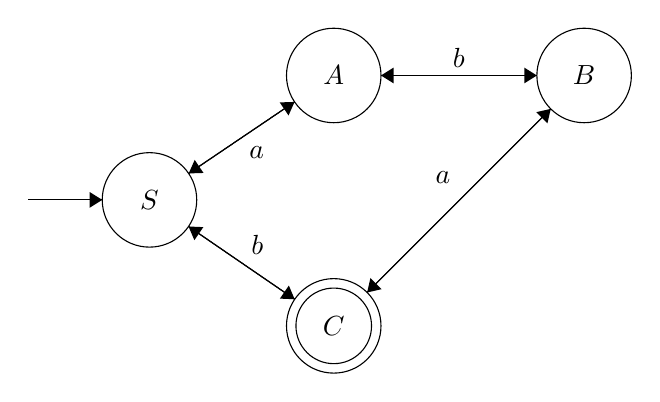
\begin{tikzpicture}[scale=0.2]
        \tikzstyle{every node}+=[inner sep=0pt]
        \draw [black] (22.9,-32.5) circle (3);
        \draw (22.9,-32.5) node {$S$};
        \draw [black] (34.6,-24.6) circle (3);
        \draw (34.6,-24.6) node {$A$};
        \draw [black] (50.5,-24.6) circle (3);
        \draw (50.5,-24.6) node {$B$};
        \draw [black] (34.6,-40.5) circle (3);
        \draw (34.6,-40.5) node {$C$};
        \draw [black] (34.6,-40.5) circle (2.4);
        \draw [black] (15.2,-32.5) -- (19.9,-32.5);
        \fill [black] (19.9,-32.5) -- (19.1,-32) -- (19.1,-33);
        \draw [black] (25.39,-30.82) -- (32.11,-26.28);
        \fill [black] (32.11,-26.28) -- (31.17,-26.31) -- (31.73,-27.14);
        \draw (29.7,-29.05) node [below] {$a$};
        \draw [black] (25.38,-34.19) -- (32.12,-38.81);
        \fill [black] (32.12,-38.81) -- (31.75,-37.94) -- (31.18,-38.77);
        \draw [black] (32.11,-26.28) -- (25.39,-30.82);
        \fill [black] (25.39,-30.82) -- (26.33,-30.79) -- (25.77,-29.96);
        \draw [black] (37.6,-24.6) -- (47.5,-24.6);
        \fill [black] (47.5,-24.6) -- (46.7,-24.1) -- (46.7,-25.1);
        \draw [black] (48.38,-26.72) -- (36.72,-38.38);
        \fill [black] (36.72,-38.38) -- (37.64,-38.17) -- (36.93,-37.46);
        \draw [black] (47.5,-24.6) -- (37.6,-24.6);
        \fill [black] (37.6,-24.6) -- (38.4,-25.1) -- (38.4,-24.1);
        \draw (42.55,-24.1) node [above] {$b$};
        \draw [black] (36.72,-38.38) -- (48.38,-26.72);
        \fill [black] (48.38,-26.72) -- (47.46,-26.93) -- (48.17,-27.64);
        \draw (42.03,-31.07) node [left] {$a$};
        \draw [black] (32.12,-38.81) -- (25.38,-34.19);
        \fill [black] (25.38,-34.19) -- (25.75,-35.06) -- (26.32,-34.23);
        \draw (29.75,-36) node [above] {$b$};
      \end{tikzpicture}
    \end{center}
  \item[b.] \hfill \\
    \begin{center}
      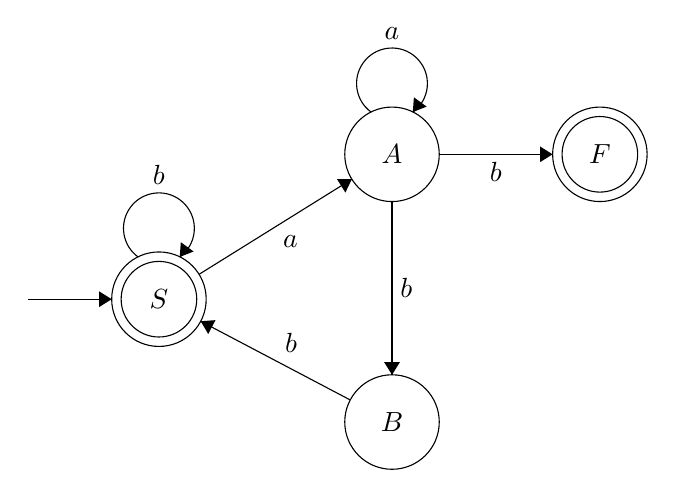
\begin{tikzpicture}[scale=0.2]
        \tikzstyle{every node}+=[inner sep=0pt]
        \draw [black] (18.2,-28.5) circle (3);
        \draw (18.2,-28.5) node {$S$};
        \draw [black] (18.2,-28.5) circle (2.4);
        \draw [black] (33,-36.3) circle (3);
        \draw (33,-36.3) node {$B$};
        \draw [black] (33,-19.3) circle (3);
        \draw (33,-19.3) node {$A$};
        \draw [black] (46.2,-19.3) circle (3);
        \draw (46.2,-19.3) node {$F$};
        \draw [black] (46.2,-19.3) circle (2.4);
        \draw [black] (16.877,-25.82) arc (234:-54:2.25);
        \draw (18.2,-21.25) node [above] {$b$};
        \fill [black] (19.52,-25.82) -- (20.4,-25.47) -- (19.59,-24.88);
        \draw [black] (9.9,-28.5) -- (15.2,-28.5);
        \fill [black] (15.2,-28.5) -- (14.4,-28) -- (14.4,-29);
        \draw [black] (20.75,-26.92) -- (30.45,-20.88);
        \fill [black] (30.45,-20.88) -- (29.51,-20.88) -- (30.04,-21.73);
        \draw (26.55,-24.4) node [below] {$a$};
        \draw [black] (33,-22.3) -- (33,-33.3);
        \fill [black] (33,-33.3) -- (33.5,-32.5) -- (32.5,-32.5);
        \draw (33.5,-27.8) node [right] {$b$};
        \draw [black] (30.35,-34.9) -- (20.85,-29.9);
        \fill [black] (20.85,-29.9) -- (21.33,-30.71) -- (21.79,-29.83);
        \draw (26.59,-31.9) node [above] {$b$};
        \draw [black] (31.677,-16.62) arc (234:-54:2.25);
        \draw (33,-12.05) node [above] {$a$};
        \fill [black] (34.32,-16.62) -- (35.2,-16.27) -- (34.39,-15.68);
        \draw [black] (36,-19.3) -- (43.2,-19.3);
        \fill [black] (43.2,-19.3) -- (42.4,-18.8) -- (42.4,-19.8);
        \draw (39.6,-19.8) node [below] {$b$};
      \end{tikzpicture}
  \end{center}  
\end{description}

\item[27.] Figure 4.33 in the book represented as a grammar.
  \begin{align*}
    A \Rightarrow&~ aB ~|~ bD ~|~ \lambda\\
    B \Rightarrow&~ aB ~|~ bC\\
    C \Rightarrow&~ aB ~|~ bC ~|~ \lambda\\
    D \Rightarrow&~ aD ~|~ bD\\
  \end{align*}
\end{description}

\end{document}
